\documentclass[a4paper, 11pt]{article}
\usepackage[top=2.5cm, bottom=2cm, left=2cm, right=2cm]{geometry} 
\geometry{a4paper} 
\usepackage[utf8]{inputenc}
\usepackage{textcomp}
\usepackage{graphicx} 
\usepackage{amsmath,amssymb}  
\usepackage{bm}
\usepackage{memhfixc} 
\usepackage{pdfsync}  
\usepackage{array}
\usepackage{xcolor}
\usepackage{tcolorbox}
\usepackage{wrapfig}
% \usepackage{fancyhdr}
% \pagestyle{fancy}


\renewcommand\thesubsection{\thesection.\alph{subsection}}
% Customization for title and author
\title{
    \vspace*{1cm} % Adjust the vertical space before the title
    \Huge CS663 - Digital Image Processing \\ % Adjust the size of the title
    \vspace{2cm} % Space between title and subtitle
    \LARGE Homework Assignment - 1 \\
    \vspace{0.2cm}
    % \Large Design Report 
    % \Large Design and Implementation Report
    \vspace{3cm}
    % \vfill
}

\author{
    Omkar Shirpure (22B0910) \\
    Aditya Saran (22B1839)\\
    Suryansh Patidar (22B1036) \\
}
\date{\vspace{3cm}August 23, 2024}

\begin{document}
\maketitle

% Insert logo at the bottom
\vfill
\begin{center}
    \includegraphics[width=0.2\textwidth]{IITB_logo.png} % Adjust the path if needed
\end{center}

\thispagestyle{empty} % Suppress page numbering on the title page

\newpage

\setcounter{page}{1} % Start numbering from the second page

\section{}
    \textbf{First Scenario:}  
    The difference in pixel sizes (0.5 × 0.5 vs. 0.25 × 0.25) suggests a uniform scaling factor in both directions (2x in both x and y directions). Affine transformations can handle scaling, rotation, translation, and shearing. So, an affine transformation would be a good motion model to align the two images.\\
    
\noindent
    \textbf{Second Scenario:}  
    Here, the pixel sizes differ in the x and y directions (0.5 × 0.5 vs. 0.25 × 0.5), indicating non-uniform scaling. Affine transformations can still accommodate this difference by applying different scaling factors along the x and y axes. As with the previous case, affine transformations are sufficient to align the images since they can model translation, rotation, and scaling, which are all that’s needed in this case.

\vspace{1cm}
\section{}
$I_1$, $I_2$, and $I_3$ are related to each other by translational motion. It is defined that:
\[
    I_j = u_{ij} I_i \quad \forall \quad i,j \in \{1,2,3\}
\]

We can write:
\[
    I_3 = u_{13} I_1 = u_{23} I_2 = u_{23} u_{12} I_1
\]

\[
    \Rightarrow u_{13} = u_{23} u_{12}
\]

During motion estimation, the above relationship holds true because any affine transformation can be decomposed into a series of more basic transformations, represented as the product of matrices. In this context, the motion from $I_1$ to $I_3$ can be expressed as a single transformation matrix or as a sequence of two transformations: first from $I_1$ to $I_2$, and then from $I_2$ to $I_3$.

\vspace{1cm}
\section{}
Looking at the coordinates from graph and MATLAB both, we can see that a point corresponding to 630 on y-axis, we get MATLAB coordinates as (135,1435) and looking at another point of value 600 on y-axis, the MATLAB coordinates are (135,969).

The difference of MATLAB's coordinates is (0,466), whereas on graph it is only 30, so there can be scaling. So for calculating the transformation matrix, we will take 3 points and assume 6 variables corresponding to affine transformation matrix and will get 6 equations to calculate all the variable of transformation matrix 

\newpage
\section{}
Dividing Equation 1 by \( f \) and Equation 2 by \( F \), we get:
\[
    \frac{x_2}{f} = \frac{a}{f}x_1^2 + \frac{b}{f}y_1^2 + \frac{c}{f}x_1y_1 + \frac{d}{f}x_1+\frac{e}{f}y_1+1
\]

\[
    \frac{y_2}{F} = \frac{A}{F}x_1^2 + \frac{B}{F}y_1^2 + \frac{C}{F}x_1y_1 + \frac{D}{F}x_1+\frac{E}{F}y_1+1
\]

Transforming into a matrix equation, we can write:
\[
    \frac{\mathbf{x_2}}{f} = \begin{bmatrix} \mathbf{x_1} & \mathbf{y_1} & 1 \end{bmatrix} \begin{bmatrix} a/f & c/f & d/f\\ 0 & b/f & e/f \\ 0 & 0 & 1 \end{bmatrix}  \begin{bmatrix} \mathbf{x_1}\\ \mathbf{y_1} \\ 1 \end{bmatrix}
\]
\[
    \frac{\mathbf{y_2}}{F} = \begin{bmatrix} \mathbf{x_1} & \mathbf{y_1} & 1 \end{bmatrix} \begin{bmatrix} A/F & C/F & D/F\\ 0 & B/F & E/F \\ 0 & 0 & 1 \end{bmatrix}  \begin{bmatrix} \mathbf{x_1} \\ \mathbf{y_1} \\ 1 \end{bmatrix}
\]

The transformation matrix consists of different affine transformations: shearing with \( \frac{c}{f} \) and \( \frac{C}{F} \), translation with \( \frac{d}{f}, \frac{e}{f} \) and \( \frac{D}{F}, \frac{E}{F} \), and scaling with \( \frac{a}{f}, \frac{b}{f} \) and \( \frac{A}{F}, \frac{B}{F} \). We can transform from \( x_1, y_1 \) to \( x_2, y_2 \) using these affine transformation matrices.

\vspace{1cm}

% \newpage
\section{} 
\subsection{}
    The MATLAB code for this part can be found in \textit{\textbf{q5.m}}
    \begin{figure}[h!] % Image environment
        \centering
        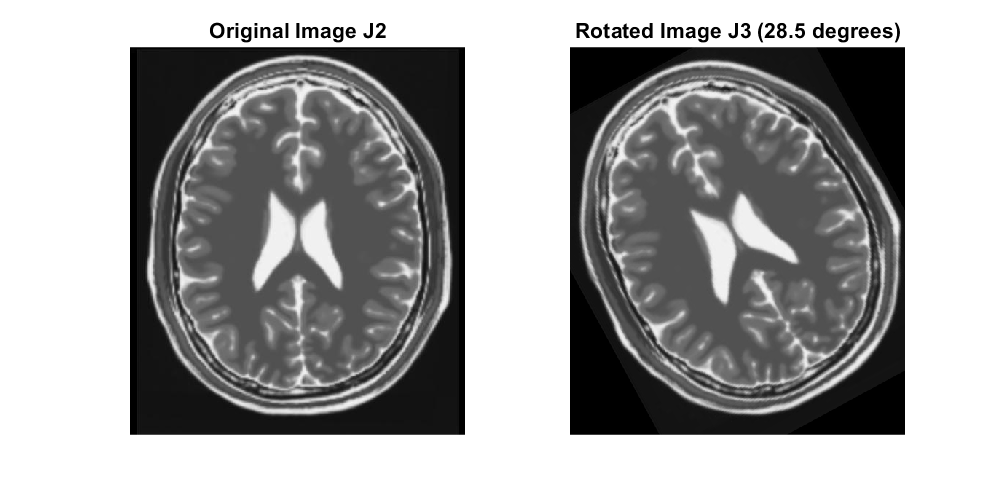
\includegraphics[width=0.6\textwidth]
        {hw1/imgs/rotated.png}
        \caption{J2 vs after rotation J2}
    \end{figure}

\subsection{}
    The MATLAB code for this part can be found in \textit{\textbf{q5.m}}
\vspace{3cm}
\subsection{}
    The plots of NCC, JE, QMI values versus $\theta$.
    \begin{figure}[h!] % Image environment
        \centering
        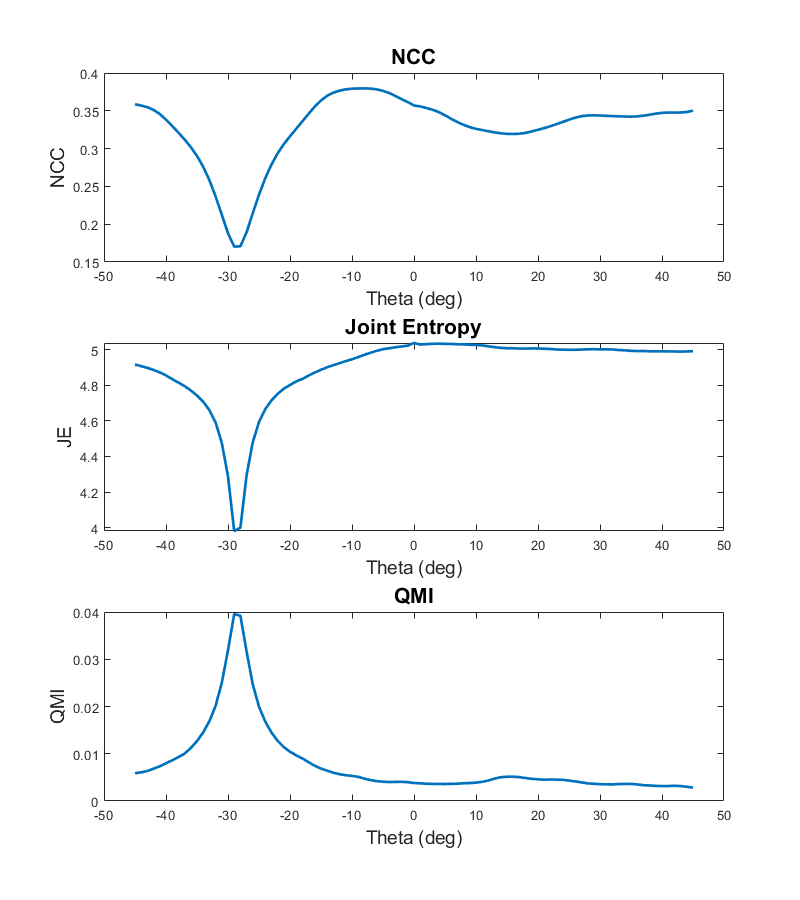
\includegraphics[width=9cm, height=10cm]{hw1/imgs/plots.png}
        \caption{Alignment comparisons with $\theta$ using NCC, Joint Entropy, QMI}
    \end{figure}
    
\vspace{1cm}
\subsection{} 
    The optimal angles obtained using different methods were as follows (negative values indicate anti-clockwise rotation): 
    \begin{itemize} 
    \item Optimal angle based on NCC: -29.0 degrees
    \item Optimal angle based on JE: -29.0 degrees 
    \item Optimal angle based on QMI: -29.0 degrees \end{itemize}

The values across all three metrics suggest that the optimal alignment between the images is achieved at a rotation of -29.0 degrees.

The minima in the NCC and JE plots indicate that, at this angle, the images are most correlated and have the least joint uncertainty, respectively. Also, the QMI plot reaches its maximum at -29.0 degrees, showing that this rotation yields the highest amount of shared information between the images.

Overall, the alignment results from the joint analysis reinforce the accuracy of the identified rotation angle of -29 degrees, providing confidence in the robustness of these metrics for determining optimal image alignment.

\newpage
\subsection{}
        \begin{figure}[h!] % Image environment
        \centering
        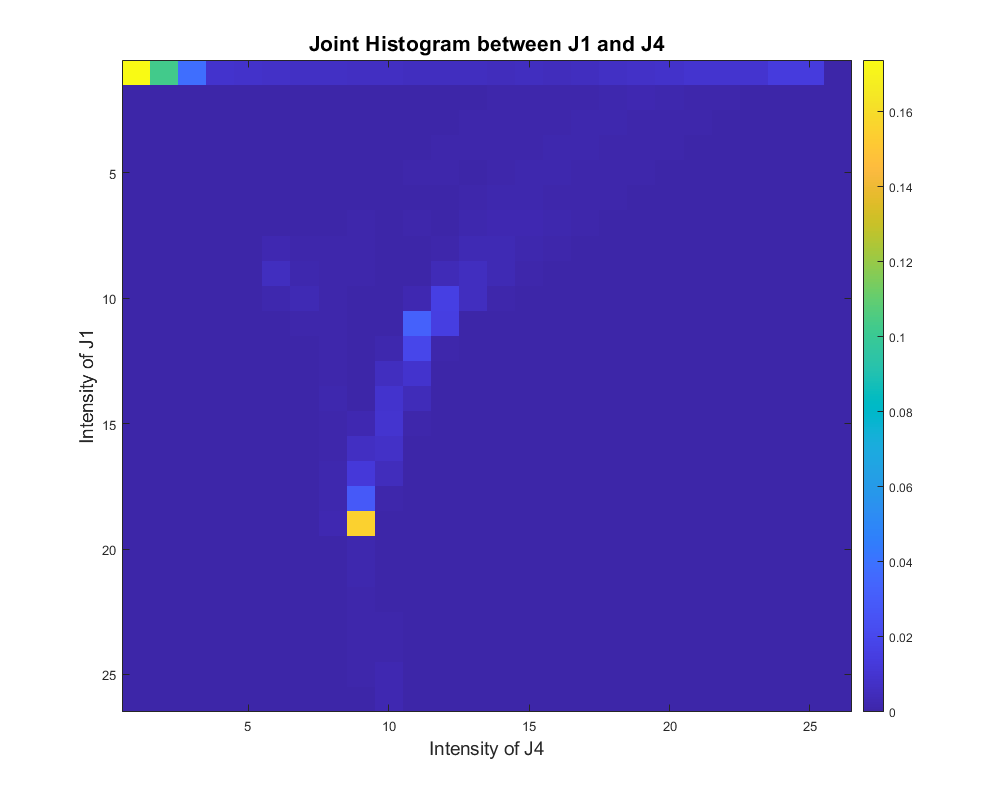
\includegraphics[width=13cm, height=10cm]{hw1/imgs/joint_intensity_hist.png}
        \caption{Joint Intensity histogram between J1 and J4}
    \end{figure}
    

\subsection{} 
The main intuition behind Quadratic Mutual Information (QMI) is to measure the shared information between the intensity distributions of two images. QMI captures how dependent the images are on each other.

When the images are well-aligned, their shared information is maximized, resulting in a higher QMI value. Statistically, if the images were dependent, they share a significant amount of mutual information, leading to a higher QMI. Conversely, if the images were independent, their joint distribution would equal the product of their marginal distributions, resulting in a QMI value close to zero. 

\[
P(I_1, I_2) = P(I_1) \cdot P(I_2)
\]

\[
QMI = \sum_{i,j} \left( P(I_1, I_2) - P(I_1) \cdot P(I_2) \right)^2
\]

\hspace{1cm}If $I_1$ and $I_2$ are independent, the term inside the summation is zero, and thus $\text{QMI}=0$.


In alignment tasks, maximizing QMI leads to the rotation angle at which the images share the most mutual information, leading to better alignment. In summary, QMI also serves as a robust measure for determining optimal image alignment. By identifying the angle (but not limited to) that maximizes QMI, we can achieve more accurate image alignment, particularly in cases where complex dependencies between the images are present.


\newpage

\section{}
\subsection{}
    Points selection in images in MATLAB code. 
\subsection{}
    The affine transformation matrix that we get from our code after choosing 12 pairs of points is,
    \[
    \begin{pmatrix}
        
        1.0244  & -0.0088  & 36.8330\\
        -0.0263  &  0.9887   &25.5556\\
         0       &  0    &1.0000\\
    \end{pmatrix}
    \]
\subsection{}

Below is three images \textit{\textbf{'goi1.jpg', 'goi2.jpg'}} and the \textit{\textbf{warped image}} after performing nearest neighbour interpolation.
\begin{figure}[h!]
    \centering
    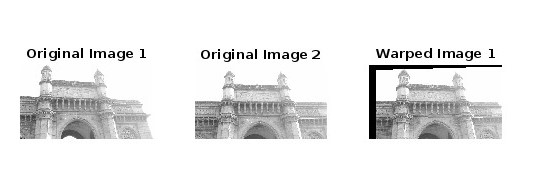
\includegraphics[width=1\textwidth]{hw1/imgs/nearest_neighbour_interpolation.jpg}
    \caption{Nearest neighbour Interpolation}
    \label{}
\end{figure}
% \vspace{6cm}

\subsection{}
Below is three images \textit{\textbf{'goi1.jpg', 'goi2.jpg'}} and the \textit{\textbf{warped image}} after performing bilinear interpolation.

\begin{figure}[h!]
    \centering
    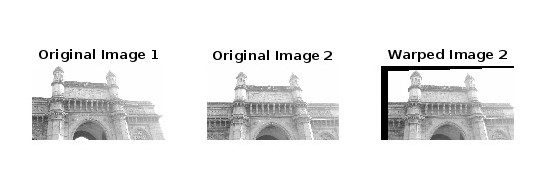
\includegraphics[width=1\textwidth]{hw1/imgs/bilinear_interpolation.jpg}
    \caption{Bilinear Interpolation}
    \label{}
\end{figure}
\vspace{2cm}
\subsection{}
If all the \textit{n} points are collinear, using any 2 points, I can write a third point and i would not have sufficient points to make a sufficient number of equations that would calculate all the unknowns of the transformation matrix, and thus we will not be able to compute our transformation matrix.

\end{document}
